
\title{Making Beautiful Graphs with Zplot}
\author{Remzi H. Arpaci-Dusseau\\
University of Wisconsin, Madison}

\begin{Abstract}

This paper introduces Zplot, a Tcl library for making two-dimensional data
plots.  Zplot provides a simple set of primitives that allow users to input
and manipulate data, plot said data in a variety of formats, and decorate the
resulting graphs with axes, labels, and other textual accents. Zplot then
outputs encapsulated postscript for ease of inclusion in technical documents.

\end{Abstract}

\section{Introduction}

Over the past 20 years or so, I have used a variety of tools to generate data
graphics for the various technical papers with which I have been
involved. These tools left me despondent. They seemed incapable of producing
all but the most basic of graphs. Many common graph types were not well
supported (e.g., bar graphs). Simple data manipulations were forced into a
long series of pre-processing steps, creating a clumsy and hard-to-maintain
tool chain. Manual manipulation on the resultant postscript was often required
to achieve the desired result.

Zplot is the fruit that was born of this frustration. Zplot is a pure Tcl
library that allows the creation of two-dimensional data graphics in a
flexible and powerful manner. Typical graphs are created with only a few lines
of Tcl, and complex and intricate graphs can be produced from only tens of
lines of code. 

In this document, I describe Zplot. First, I will give an overview of the tool
and the basic primitives it provides. Then, I will describe each of the basic
routines in more detail, showing how they can be combined to produce a wide
range of interesting graphs. Zplot drawing routines are all built upon a set
of low-level postscript-generating commands; these hide many of the details of
generating correct postscript from the rest of Zplot, boiling down most
activies to simple drawing commands that place lines, shapes, and text on the
drawing surface. 


\section{Overview}

I now describe the basic primitives provided by Zplot. Let us start with a
typical (if simple) graph as an example, and use this to drive the discussion
of the different elements of Zplot. A typical graphing script might be written
as follows:

\begin{verbatim}
# input the library
source zplot.tcl
namespace import Zplot::*

# describe the drawing surface
PsCanvas -title "file.eps" -width 300 -height 200
  
# load some data
Table -table t -file "file.data" 

# make a drawable region for a graph
Drawable -xrange 0,10 -yrange 0,20

# make some axes
AxesTicsLabels -title "A Sample Graph" -xtitle "The X-Axis" -ytitle "The Y-Axis"

# plot the points
PlotPoints -table t -xfield x -yfield y -style triangle -linecolor red

# finally, output the graph to a file
PsRender -file "file.eps"
\end{verbatim}

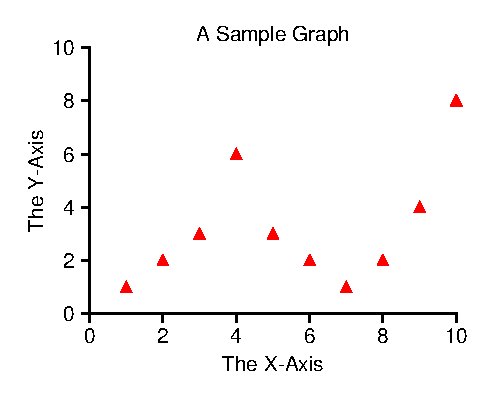
\includegraphics{first-example.eps}

In this example, the user creates a graph by first describing the drawing
surface by calling \texttt{PsCanvas} and giving it a height and width. Then,
the user calls the \texttt{Table} routine to load data into Zplot, getting the
data from a file (file.data). The user, wishing to plot the data, now creates
a drawable region by calling the \texttt{Drawable} routine; doing so defines
where on the canvas the drawable is, and also how to map data points onto the
drawing surface (e.g., the range of x values and y values that map onto this
drawable). With a drawable defined, the user can now call one of a variety of
plotting routines (e.g., \texttt{PlotPoints}) to plot the data onto the
drawable. The plotting routines generally take a large number of arguments,
enabling a wide variety of plots to be produced; in this case, the user
chooses to draw a red triangle at each (x,y) point of the graph. Finally, the
user adds some graphical and textual decorations to help clarify the graph (in
this case, by simply calling the \texttt{AxesTicsLabels} routine), and then
renders the postscript to a file by calling PsRender.  We now describe each of
these primitives (and a few others) in turn.

Note that each of these routines takes a large number of optional parameters.
To find out what these are (without perusing the source code), simply call the
routine and pass it the ``-help'' flag (or any bad flag); a useful error
message about the routine and all of its parameters (including default values)
will be printed to the console.

\subsection{Table}

There are numerous routines available to users to input and manipulate data;
these are known as the \texttt{Table*} routines. The most commonly used
routine is the basic \texttt{Table} routine; usually, this routine is used to
input a file and then plot its points. A typical file (such as ``file.data''
above) looks like this:
\begin{verbatim}
# x y
0 0 
1 1 
2 2 
3 3 
4 6 
5 3 
6 2 
7 1 
8 2 
9 4 
10 8
\end{verbatim}
The first line contains the ``schema'' for the table, with names for each
column; these names are subsequently used to refer to the data when
manipulating it or drawing it to the screen. When there are no names specified
on the first line, Zplot uses c0,c1,...,cN as default names.

One powerful routine is the \texttt{TableSelect} command; it allows one to
perform a database-like selection over a table and put the results in a new
table. Here is an example that selects data from table ``t'' with y-values
above 5, and plots green circles around said points:
\begin{verbatim}
Table -table thi -columns x,y
TableSelect -from t -to thi -where {\$y > 5}
PlotPoints -table thi -xfield x -yfield y -style circle -linecolor green -size 4 -linewidth 0.25
\end{verbatim}

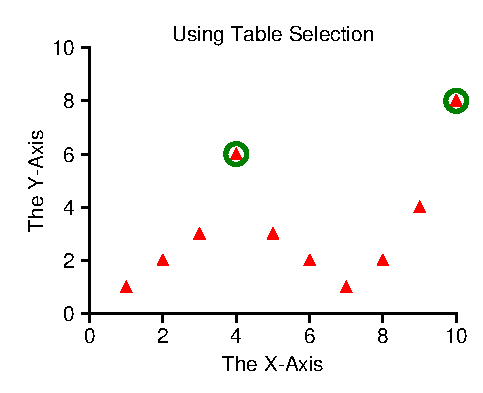
\includegraphics{second-example.eps}

There are a number of other useful table functions which are not covered here,
mostly for manipulating and summarizing data. For example, \texttt{TableMath}
can be used to perform a mathematical operation (or indeed, any valid Tcl
expression) on a column of data. The routine \texttt{TableComputeMeanEtc} is
useful for computing means and deviations over a column, and
\texttt{TableBucketize} can be used to place data into bins. All of these
primitives are built on lower-level table routines that access each row of a
table and perform operations on its contents; thus, more complex operations on
tables can be readily assembled by adventurous users.

\subsection{Drawable}

The drawable is likely the most important abstraction that Zplot implements. A
drawable is created by the \texttt{Drawable} command. Each drawable has a
name; the default name is ``default'' and this default is used by all routines
that expect a drawable unless otherwise specified. Here is the relevant
portion of the example above rewritten to use the drawable name ``foo''
instead of the default:

\begin{verbatim}
Drawable       -drawable foo -xrange 0,10 -yrange 0,20
AxesTicsLabels -drawable foo -title "A Sample Graph" -xtitle "The X-Axis" -ytitle "The Y-Axis"
PlotPoints     -drawable foo -table t -xfield x -yfield y -style triangle -linecolor red
\end{verbatim}

The powerful aspect of a drawable is that it enables a user to place multiple
(potentially overlapping) drawable regions onto the drawing surface. This
feature can be used to implement a number of interesting graphs. For example,
in this graph (taken from ~\cite{SivathanuEtAl04-DGRAID}), two regions of the
graph are of interest but hard to see due to their small size. Thus, we create
two additional drawables and plot closeups of the data in those regions:

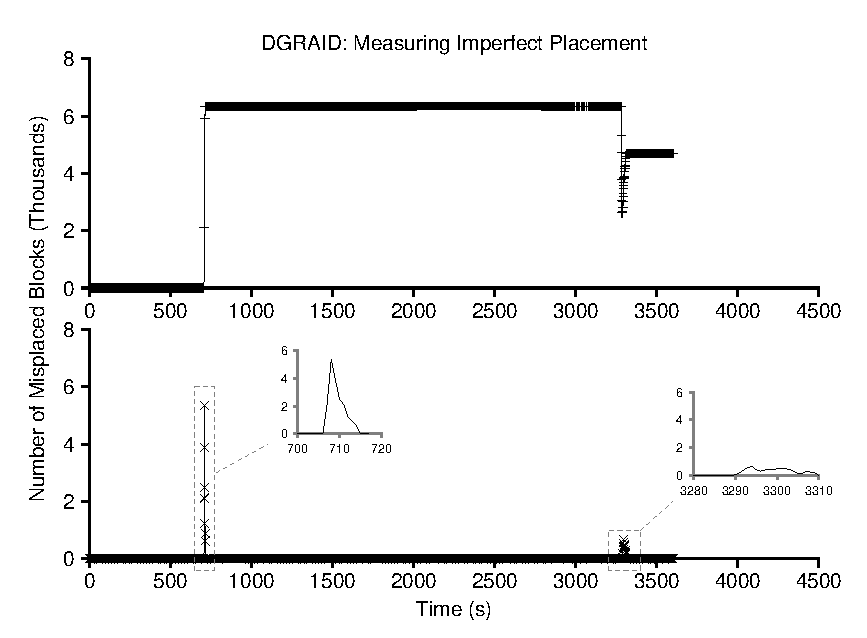
\includegraphics{dgraid.eps}

These types of closeups are trivial to implement. Here is the code for one of
them (the entire example, and many others, can be found on the Zplot web
site):

\begin{small}
\begin{verbatim}
Drawable -drawable copyc1 -xoff 135 -yoff 90 -height 40 -width 40 \
    -xrange 700,720 -yrange 0,6000
Table -table copyc1 -columns c0,c1
TableSelect -from copy -to copyc1 -where {($c0>=700) && ($c0<=720)}
AxesTicsLabels -drawable copyc1 -ticmajorsize 2 -xauto ,,10 -yauto ,,2000 \
    -ylabeltimes 0.001 -ylabelformat "\%d" -linecolor gray -fontsize 6
PlotLines -drawable copyc1 -table copyc1 -xfield c0 -yfield c1 -linewidth 0.25
\end{verbatim}
\end{small}

This example also demonstrates a number of parameters that the
\texttt{Drawable} routine can be passed. For example, a user can specify its
exact position with the ``xoff'' and ``yoff'' flags, and its dimensions with
the ``width'' and ``height'' parameters. 

%Example: 
% - multiple graphs on same canvas (side by side)
% - small drawable on big drawable (enables closeups)
% - multiple overlapping drawables (enables different y-axes)

Multiple drawables can also be used to plot data with multiple y axes in a
simple and straightforward manner. In this example, we plot the same data from
the example above, except onto an overlapping drawable that maps the y range
from 0 up to 20 (instead of 0 to 10). The code is below; the resulting graph
thus plots the same data twice, once in red (as relative to the left y-axis),
and once in green (as relative to the right).

\begin{verbatim}
Drawable -drawable second -xrange 0,10 -yrange 0,20 -width 230
AxesTicsLabels -drawable second -style y -ytitle "Second Y-Axis" \
    -labelstyle in -yaxisposition 10 -yauto ,,4 -ticstyle in
PlotPoints -drawable second -table t -xfield x -yfield y \
    -style triangle -linecolor green -fill t -fillcolor green
\end{verbatim}

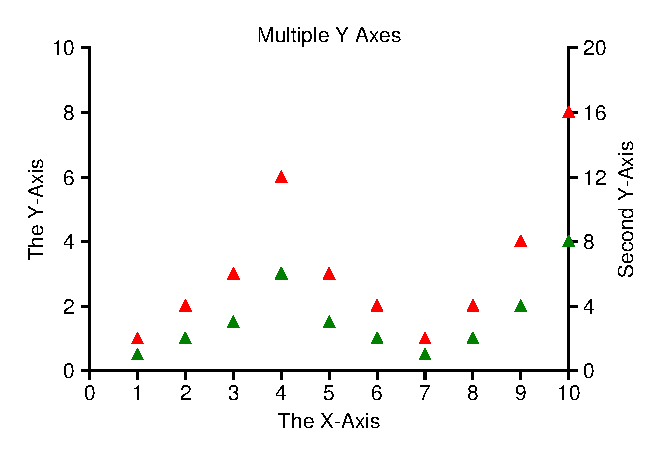
\includegraphics{third-example.eps}

Thus, the drawable is a powerful abstraction for drawing data graphics. 

\subsection{The Plot* Family}

There are currently eight members in the \texttt{Plot*} family:
\texttt{PlotHeat}, \texttt{PlotVerticalBars}, \texttt{PlotHorizontalBars},
\texttt{PlotVerticalIntervals}, \texttt{PlotHorizontalIntervals},
\texttt{PlotPoints}, \texttt{PlotLines}, and \texttt{PlotVerticalFill}.
Most should be self explanatory from the name, and examples of each can be
found in the figure below.

Many ideas were stolen here from Ploticus~\cite{Ploticus}, an excellent
graphing tool (discussed further in Section~\ref{sec-related}). 



There is also a plotting function that takes an equation instead of a
table: \texttt{PlotFunction}. ...




\subsection{Axes, Tics, and Labels}



\subsection{Legend}



\section{Postscript: Understanding The Heart of Zplot}
\label{sec-ps}

\newcommand{\psline}{\texttt{PsLine}}
\newcommand{\psbox}{\texttt{PsBox}}
\newcommand{\pstext}{\texttt{PsText}}

Zplot is built on top of a number of underlying postscript primitives,
including basic lines, filled (or empty) shapes, and text. Each of these
routines is used by the plotting routines and other entities that wish to
create pictoral or textual elements upon on the drawing surface. We now
describe the primitives in turn.

\begin{verbatim}
PsLine -coord <x1,y1:x2,y2:...:xN,yN> (in pts)
       -linecolor <color> 
       -linewidth <width in pts>
       -linecap <0, 1, or 2>
       -linejoin <0, 1, or 2>
       -linedash <dash pattern>
       -closepath <true or false>
\end{verbatim}



The \psline\ primitive is passed a set of coordinates, some basic information
about the line, and then produces a line that connects the coordinates in the
resulting postscript. All postscript primitives take coordinates in postscript
``ems'', each of which is 1/72nd of an inch. Figure~\ref{fig-psline} shows how
the parameters of the \psline\ command affect the resulting output.

The \psline\ primitive also takes additional arguments that allow the addition
of an arrow to the end of the line; we omit these parameters for the sake of
space. Future work will likely support a broader set of annotation tools such
as this.



\begin{verbatim}
PsBox -coord x1,y2:x2,y2
PsCircle -coord x,y -radius r
PsPolygon -coord x1,y1:...:xN,yN
    -linecolor 
    -linedash 
    -linecap 
    -fill <true or false>
    -fillcolor <color of each element>
    -fillstyle <style>
    -fillsize <size of each element in pattern>
    -fillskip <amount to skip between each element in pattern>
    -fillshift <+x,+y>
    -bgcolor <color of background behind pattern>
\end{verbatim}

Each of these take a variety of arguments that describe their coordinates,
and then all take three different sets of arguments that characterize the line
around the shape (-line*), the fill of the shape (-fill*), and the background
color behind the shape (-bgcolor). The line descriptors match those of
\psline\ above, and the background color is straightforward. Most interesting,
then, is the variety and flexibility provided by the pattern descriptions.

% Patterns
The -fill* parameters allows users to specify a fill pattern for a region. The
most important parameter is \texttt{-fillstyle}, which determines how the
region is filled. Current styles that are supported include \textt{solid,
hline, vline, dline1, dline2, circle, square, triangle, utriangle}; more are
added occasionally (when the author needs them). Each pattern takes two
arguments to determine its contents: \texttt{-fillsize} and
\texttt{-fillskip}. Within a given pattern, \texttt{-fillsize} determines 
the size of each element in the pattern, and \texttt{-fillskip} the space
between each element. 

Figure xxx ...

\includegraphics{pattern-example.eps}

\begin{verbatim}
PsText -coord <x,y>
       -text <the string of text to write on the canvas>
       -font <font choice>
       -color <color>
       -rotate <angle of rotation>
       -anchor <how to anchor the text>
       -bgcolor <a background color behind the text>
       -bgborder <how big the color border should be around the text>
\end{verbatim}

The last primitive we describe is \pstext, which draws text onto the
screen. Most of its parameters are straightforward. However, the most crucial
argument to understand is the \texttt{anchor}. This parameter describes how
the text should be anchored relative to the coordinate that was passed to the
routine. The parameter takes the form <xanchor,yanchor>, where xanchor
specifies the anchoring of the text in the x direction (either l for left, c
for center, or r for right), and yanchor the anchoring in the y direction (l
for low, c for center, and h for high). Figure~\ref{fig-pstext} shows the
different possible anchors (with the coordinate highlighted with a red
circle).  

\begin{}
% 
\includegraphics{anchor-example.eps}
\end{}


\section{Examples}





\section{Limitations}


Postscript: simple but often inefficient.



Error reporting: 
OK at a high level
(when passing bad flags to an exported routine, say)
Bad at type checking (is this really an int, say)






\section{Performance Evaluation}

``The fast drives out the slow, even if the fast is wrong.'' (W. Kahan)

Tcl is slow. Thus, Zplot is slow. If you try to manipulate millions of data
points, you will have to wait for a while, even on a modern processor. The
graph below (yes, produced by Zplot!), shows the time it takes to generate a
scatterplot of varying sizes. As one can see from the graph, ...

Of course, Zplot was not written with optimized performance in mind (of
course, it was not written to be horrifically slow, either). 

Ironically, John Ousterhout's paper ``Why are Operating Systems ...''  points
out many reasons that operating system functions don't scale with processor
performance improvements as one might expect; similar arguments can be made
about Tcl. Although processors have improved greatly in the past 10 years, Tcl
remains slow in both a relative and absolute sense. It is this author's
opinion that this fundamental performance flaw has kept Tcl from being more
broadly accepted, and has thus paved the way for other scripting languages to
overtake it in terms of popularity and user base (\eg, Python~\cite{Python}).

\subsection{Commenting on Tcl}



Namespaces:
Quite nice, simple and powerful.
Wish it had been there earlier.

Packages:
still don't like it, generally don't use it.
Just makes things more of a pain.

Performance:
As above. Too slow.


\section{Related Work}

Much of the frustration I spoke of earlier was with a tool known as
gnuplot~\cite{gnuplot}. Gnuplot provides excellent support for simple line
graphs and scatter plots, as well as numerous other graph types. However, its
lack of any reasonable support for bar charts was one of the main driving
forces behind Zplot. However, I should note that the postscript produced by
gnuplot was clear and easy to read, sparking my interest in that language, and
thus (indirectly) making Zplot possible.

As I demonstrated Zplot to others, many people referred me to
Ploticus~\cite{Ploticus}, which is a more powerful and complete tool than
gnuplot and is capable of producing a large variety of interesting graph
types. Many of the features found in Zplot are also found in Ploticus (e.g., a
ploticus ``area'' is akin to a Zplot Drawable), and I often found myself
downloading examples from the Ploticus web page to see if Zplot could easily
do what Ploticus already does. Indeed, at one point I even considered dropping
Zplot development and simply adding a few features to Ploticus that I found
lacking (\eg, bar graphs with a variety of pretty patterns). However, one look
at the Ploticus source code convinced me I was on the right path. Ploticus is
comprised of over 60,000 lines of C code. Zplot, in contrast, is less than
5,000 lines of Tcl; although not always beautiful, certainly quite a bit
simpler. This comparison is a bit unfair, as Zplot is not (yet!) as powerful
as Ploticus, but I feel quite positive that it will never be nearly as large,
a testimony to the power of the Tcl language.

There are a number of other plotting packages out there as well. Jgraph, BLT, ...


\section{Conclusions}
















